\chapter{Results and Discussion}

This is how we do it! \myworries{Still to do here}
\section{Piezo and the extracellular matrix}

Main Insights:
\begin{itemize}
    \item Intracellular protein much lower even three days after intervention. Two possible explanation: Either protein synthesis normal, but continuously depleted (Piezo1-Activation as release mechanism)  or protein production is halted
    
    \item Secretome is really intersting, gives some hits that can be confirmed using small-scale readouts. \texttt{>} COL1A1, IL6
    
    \item Col1a1 in PCR significantly different three days after intervention. Tendency already visible in d2. Likely significant with increasing sample size, since Western Blots afterwards imply linear effect growth.
    
    \item If you follow second hypothesis, then it seems like Protein precedes RNA representation (weird!) and there must be something between RNA and Protein that, in response to Piezo1 activation, degrades Protein (EVEN WEIRDER)
    
     \item  Caveat: Likely differentiation during experiment. FGF-2 (dedifferentiation factor, known for suppressing ECM-production \myworries{[citation needed]}) not present during experiment, but during whole cell culture. Same thing with FBS. 
     
    \item Caveat: We compare against cells that have already spent 8-14h in serum free media (read: FGF-2 free).    
    
    \item Caveat: Cells die after Yoda1-Intervention
    
    \item Courtesy of Uli: The effect is very likely Piezo1 dependent. Western Blot of Knock-outs and NoT show clearly disappearing Collagen 1 after Yoda adiminstration only in NoT. 
    
    \item Calcium signal: Fluidic shear leads to strong calcium signal in cells. We show that it is definitely extracellular influx in cells (through functionalization of medium, as opposed to release of Ca2+ from the ER). Second through experiments with KO's, we show that this is Piezo1 mediated. 
\end{itemize}

\begin{figure}[h!]
    \centering
    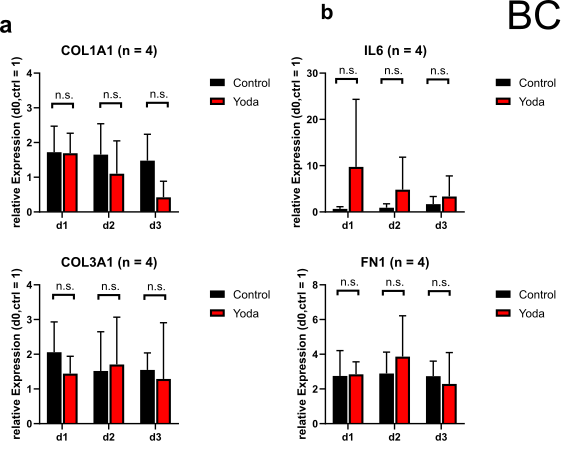
\includegraphics[scale = 0.6]{Collection.png}
    \caption{
    PCR Experiments where we saw some really cool stuff happening. \textbf{a}: Col1$\alpha$1 output \textit{(n = 4)}
    }
    \label{fig:my_label}
\end{figure}

\subsection{WesternBlot}

\kant[42]
\subsection{qRT-PCR}

\section{Piezo1 as integrator of biomechanical events}
\myworries{Worries}
\subsection{Functionalization of Medium}
\subsection{Piezo1 as main integrating receptor}

\section{Biostability of Yoda1}
\kant[42][1-3]